\subsection*{Problema 26}

\textbf{Enunciado:}
Calcular la integral indefinida:
\begin{align*}
\int \dfrac{2x^2 - 3x + 5}{(x + 2)(x - 1)(x - 3)} \, dx
\end{align*}

\textbf{Solución:}
El integrando es una función racional propia. Aplicamos el método de fracciones parciales. Suponemos la descomposición:
\begin{align*}
\dfrac{2x^2 - 3x + 5}{(x + 2)(x - 1)(x - 3)} = \dfrac{A}{x + 2} + \dfrac{B}{x - 1} + \dfrac{C}{x - 3}
\end{align*}

Multiplicamos toda la ecuación por el denominador común $(x + 2)(x - 1)(x - 3)$:
\begin{align*}
2x^2 - 3x + 5 &= A(x - 1)(x - 3) \\
&+ B(x + 2)(x - 3) \\
&+ C(x + 2)(x - 1)
\end{align*}

Para hallar las constantes, evaluamos en las raíces del denominador:
Si $x = -2$:
\begin{align*}
2(-2)^2 - 3(-2) + 5 &= A(-3)(-5) \\
8 + 6 + 5 &= 15A \implies 19 = 15A \\
A &= \dfrac{19}{15}
\end{align*}

Si $x = 1$:
\begin{align*}
2(1)^2 - 3(1) + 5 &= B(1 + 2)(1 - 3) \\
2 - 3 + 5 &= B(3)(-2) \\
4 &= -6B \implies B = -\dfrac{2}{3}
\end{align*}

Si $x = 3$:
\begin{align*}
2(3)^2 - 3(3) + 5 &= C(3 + 2)(3 - 1) \\
18 - 9 + 5 &= C(5)(2) \\
14 &= 10C \implies C = \dfrac{7}{5}
\end{align*}

Sustituimos los valores de $A$, $B$ y $C$ en la integral:
\begin{align*}
\int &\left[ \dfrac{19/15}{x + 2} - \dfrac{2/3}{x - 1} + \dfrac{7/5}{x - 3} \right] dx
\end{align*}

Integramos cada término utilizando logaritmos naturales:
\begin{align*}
&= \dfrac{19}{15} \ln|x + 2| - \dfrac{2}{3} \ln|x - 1| \\
&+ \dfrac{7}{5} \ln|x - 3| + C
\end{align*}

\begin{figure}[H]
	\centering
	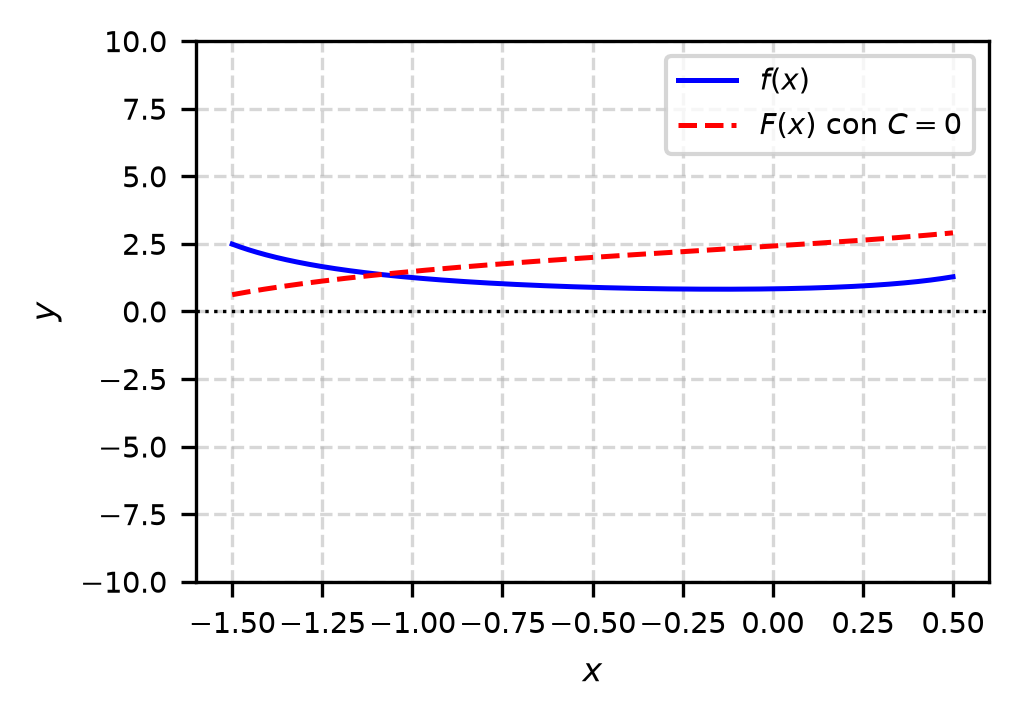
\includegraphics[width=\columnwidth]{semana_03/graficas/SEM03_P26_grafica.png}
	\caption{Representación gráfica de $f(x)$ y su antiderivada $F(x)$ evaluada para la constante de integración $C = 0$ (Problema 26).}
	\label{fig:problema26}
\end{figure}
